\documentclass[twocolumn, 12pt]{article} % 小四约等于12pt

% --- 基础宏包 ---
\usepackage{xeCJK} 
\usepackage{fontspec} 
\usepackage{amsmath, amssymb} 
\usepackage{geometry} 
\usepackage{graphicx} 
\usepackage{float} 
\usepackage{booktabs} 
\usepackage{array}
\usepackage{titlesec} 
\usepackage{abstract} 
\usepackage{caption}
\usepackage{subcaption}
\usepackage{enumitem}

% --- 字体设置 ---
% 请确保系统已安装 SimSun (宋体) 和 Times New Roman
\setCJKmainfont[BoldFont=SimHei]{SimSun} % 中文宋体，加粗用黑体
\setmainfont{Times New Roman} % 西文 Times New Roman

% --- 页面布局 ---
\geometry{a4paper, left=2cm, right=2cm, top=2.5cm, bottom=2.5cm}

% --- 标题格式定制 ---
\titleformat{\section}{\large\bfseries}{}{0em}{}
\titleformat{\subsection}{\normalsize\bfseries}{}{0em}{}
\titleformat{\subsubsection}{\normalsize\bfseries}{}{0em}{}

% --- 字号命令 ---
\newcommand{\xiaosi}{\fontsize{12pt}{15pt}\selectfont} % 小四
\newcommand{\wuhao}{\fontsize{10.5pt}{12.6pt}\selectfont} % 五号

% --- 标题信息 ---
\title{\textbf{基于熵权自适应粒子群算法与神经网络的最速降线轨迹优化研究}}
\author{}
\date{}

\begin{document}
	
	% --- 摘要与关键词 (单栏) ---
	\twocolumn[
	\begin{center}
		\maketitle
		\xiaosi 姓名：林鑫 \quad 班级：信计2302班 \quad 学号：1043220122
	\end{center}
	\noindent\xiaosi\textbf{摘要：} 最速降线问题是变分法与最优控制领域的经典课题。尽管在理想环境下存在解析解（摆线），但在引入摩擦力、空气阻力及离心力等复杂动力学约束的非保守物理场中，解析法往往很难求解。本文提出了一种结合物理信息神经网络（PINNs）与熵权粒子群算法的混合优化框架。首先，利用神经网络对路径进行参数化，并引入严格的数学拟设机制强制消除边界误差，将有约束优化转化为无约束优化。其次，针对物理损失函数高度非凸、易陷入局部最优的问题，提出了一种熵权自适应粒子群算法。该算法通过香农熵实时量化种群多样性，动态调节搜索策略。基于可微分物理引擎的仿真结果表明，在含非线性阻力与离心力，摩擦力的复杂场中，本文方法不仅能精准复现理想解，更能智能权衡"速度收益"与"能量损耗"，寻找到优于传统数值方法的物理可行解。
	\par \vspace{1em}
	\textbf{关键词：} 物理信息神经网络 (PINNs); 熵权自适应; 粒子群算法; 复杂动力学约束; 轨迹优化
	\vspace{2em}
	]
	
	\xiaosi % 正文小四
	
	\section{1. 引言}
	\subsection{1.1 经典问题与现实挑战}
	自 1696 年 Johann Bernoulli 提出最速降线问题以来，其在重力场下的解析解——摆线，已成为物理学的经典结论。然而，随着无人机（UAV）自主导航、工业机械臂轨迹规划以及高速运输系统设计等现代工程需求的出现，传统的理想化模型面临严重挑战。在现实场景中，质点不仅受重力影响，还受到与速度平方成正比的非线性空气阻力、摩擦力以及运动路径弯曲产生的离心力影响。在这些非保守力场中，能量不再守恒，系统展现出高度的非线性和非凸性，使得解析推导变得异常困难，通常需要借助数值优化手段进行求解 [1]。
	
	\subsection{1.2 现有方法的局限性}
	目前的求解方法主要分为两类，但各具局限：\\
	1）传统数值法（如直接配点法）： 极度依赖离散化精度。若采样点不足，生成的轨迹缺乏光滑性，且在处理起点导数奇异性（垂直下落）时易产生数值失真。\\
	2）深度学习方法（如 PINNs）： 虽然能提供连续光滑的解，但其物理损失函数通常具有高度非凸。传统的梯度优化器（如 SGD、Adam）在处理此类长程物理积分约束时，极易陷入局部极小值或遭遇梯度消失。\\
	3）标准群智能算法（如 PSO）： 虽然具备全局搜索能力，但其控制参数固定，在搜索后期容易发生“早熟收敛”，无法在复杂的物理空间中实现高精度微调。
	
	\subsection{1.3 相关工作与文献综述}
	针对轨迹优化问题，Raed Abu Zitar [2] 探索了监督学习与强化学习神经网络在捕捉最速降线路径中的潜力，证明了神经网络在捕捉控制规律方面的优越性。而在全局寻优算法方面，粒子群算法（PSO）的应用十分广泛。为了提升 PSO 在复杂搜索空间中的效率，Zhan 等人 [4] 提出了自适应粒子群算法（APSO），通过进化状态估计（ESE）实时识别种群状态并调节参数。本文结合这一思路，进一步引入信息熵辅助策略来维护种群多样性 [5]，通过熵值的连续反馈实现更精准的“收敛-发散”切换，为解决复杂环境下的轨迹搜索提供了理论支撑。
	
	\subsection{1.4 研究目标与主要贡献}
	本文的主要贡献如下：\\
	1）基于Ansatz硬约束的神经路径参数化：我们并未简单地将神经网络输出作为路径点，而是设计了一种特殊的数学结构，将线性基线与网络输出的非线性偏差相结合，通过乘以边界因子，从数学上强制保证了所有生成的轨迹严格满足起始点 (0,0) 和终点 ($x_{end}, y_{end}$) 的边界条件。这极大地压缩了搜索空间，提高了优化的有效性。\\
	2）熵权驱动的自适应参数调节机制：针对 PSO 的早熟问题，我们引入了信息熵的概念来度量粒子群的“混乱度”或“多样性”。不同于传统的标准差度量，本文通过对各维度粒子位置进行归一化并构建一维直方图，计算其香农熵的均值来实时感知当前的搜索状态。基于这一熵值，我们设计了一套自适应规则，动态调整惯性权重 (w) 和认知/社会学习因子 ($c_1, c_2$)，在低多样性时增强探索，在高多样性时加速收敛。\\
	3）可微分物理引擎的构建：我们实现了一个基于PyTorch的可微分物理引擎。该引擎不仅能计算保守场下的能量守恒，还能通过递归方式求解非保守场（含摩擦和阻力）中的动能定理，实现了从路径几何到物理耗时的端到端梯度传播。\\
	4）算法改进后的仿真：我们改进后的Entropy-PSO在求解最速降线问题上的表现，验证了改进算法在收敛精度、收敛速度及跳出局部最优能力上的显著优势。
	
	\section{2. 问题描述与数学建模}
	\subsection{2.1 广义最速降线问题的物理模型}
	考虑一个质点在重力场中从点 A(0,0) 运动到点 B($x_{end}, y_{end}$)。在本文的坐标系定义中，为了方便物理计算，我们通常取 y 轴向下为正（但在可视化时会进行翻转以符合直观视觉）。
	
	\subsubsection{2.1.1 理想情况（Conservative Field）}
	在无摩擦、无阻力的理想情况下，系统的机械能守恒。假设初速度为0，质点在垂直高度 y 处的速度 v 仅由势能转化为动能决定：
	\begin{equation}
		\frac{1}{2}mv^2 = mgy \Rightarrow v(y) = \sqrt{2gy}
	\end{equation}
	此时，目标是最小化总时间泛函 J[y]：
	\begin{equation}
		J[y] = \int_{0}^{x_{end}} \frac{ds}{v} = \int_{0}^{x_{end}} \sqrt{\frac{1+(y'(x))^2}{2gy(x)}} dx
	\end{equation}
	这就是经典的欧拉-拉格朗日方程求解对象，其解析解为摆线。
	
	\subsubsection{2.1.2 复杂物理场（Non-Conservative Field）}
	在实际工程问题中，必须考虑非保守力。假设存在动摩擦系数 $\mu$ 和空气阻力系数 $C_d$ (Drag Coefficient)。\\
	1）摩擦力：$f_f = \mu N$。其中法向力 N 不仅包含重力的分量 $mg\cos\theta$，还包含由于路径弯曲产生的离心力（Centrifugal Force）：
	\begin{equation}
		N = mg\cos\theta + m\frac{v^2}{R}
	\end{equation}
	其中 R 是曲率半径，$\theta$ 是路径切角。路径曲率 $\kappa = 1/R$ 定义为：
	\begin{equation}
		\kappa(x) = \frac{|y''|}{(1+(y')^2)^{3/2}}
	\end{equation}
	2）空气阻力：假设阻力与速度平方成正比，即 $F_d = \frac{1}{2}\rho C_d A v^2$，在归一化模型中，我们将共简化为 $F_{drag} = k_{drag}v^2$。\\
	在非保守场中，速度 v 不再是位置的单值函数，而是路径积分的结果。根据动能定理，动能的增量等于合外力做的功：
	\begin{equation}
		d(\frac{1}{2}mv^2) = (mg\sin\theta - f_f - F_d)ds
	\end{equation}
	\begin{equation}
		v \cdot dv = (g\frac{dy}{ds} - \mu(g\frac{dx}{ds} + \kappa v^2) - \frac{k_{drag}}{m}v^2)ds
	\end{equation}
	优化目标依然是最小化时间 $T = \int dt$，但此时必须满足上述复杂的微分代数方程约束。
	
	\subsection{2.2 神经网络路径参数化与Ansatz约束}
	为了求解上述泛函极值问题，我们采用神经网络 $N(x;\theta)$ 来参数化路径 $y(x)$。相比于多项式逼近或离散点表示，神经网络具有更强的非线性表达能力。
	然而，普通的神经网络输出很难精确满足端点约束 $y(0)=0$ 和 $y(x_{end})=y_{end}$。软约束往往导致边界处存在微小误差，这在物理积分中是不可接受的。因此，本文采用了 Ansatz（拟设）硬约束技术。我们将最终的路径输出 y(x) 定义为：
	\begin{equation}
		y(x) = \frac{y_{end}}{x_{end}} \cdot x + x \cdot (x - x_{end}) \cdot N(x; \theta)
	\end{equation}
	其中，第一项为线性偏置（Linear Bias），第二项包含边界因子（Boundary Factor）。通过这种构造，无论神经网络的参数 $\theta$ 如何变化，函数 $y(x)$ 在端点处的值始终固定为预设值。从而将有约束优化问题转化为无约束优化问题，大大降低了求解难度。
	
	\section{3. 算法原理与改进：熵权自适应粒子群算法}
	\subsection{3.1 标准粒子群算法（PSO）及其局限性}
	标准 PSO 算法通过模拟鸟群的捕食行为来寻找最优解。粒子的速度和位置更新公式如下：
	\begin{equation}
		v_i^{t+1} = wv_i^t + c_1r_1(pbest_i - x_i^t) + c_2r_2(gbest - x_i^t)
	\end{equation}
	\begin{equation}
		x_i^{t+1} = x_i^t + v_i^{t+1}
	\end{equation}
	局限性分析：对于高维非凸的神经网络权重空间，固定的参数往往导致勘探不足（Under-exploration）或开发不足（Under-exploitation）。
	
	\subsection{3.2 引入熵权的多样性度量}
	1）群体多样性与信息熵
	参考相关研究 [5] 提出的熵辅助策略，本文将搜索空间划分为 M 组等分网格，计算微粒在权值空间中的分布熵 H。该机制能有效表征种群的聚类程度，弥补了传统 APSO 在处理高维权值空间时对多样性感知不足的缺陷 [4]。
	表 1：熵权自适应规则矩阵
	
	2）熵权的搜索隐喻
	借鉴 Gao 等人 [5] 的熵辅助（Entropy-Assisted）逻辑，本文设计了基于熵权的动态调节机制。当阈值指示种群陷入局部最优时，算法模仿 Zhan [4] 提出的跳出机制，通过调整惯性权重 w。此外，方伟等人 [6] 提出的多样性控制 PSO (DCPSO) 为本文在复杂物理场下处理“收敛-发散”平衡提供了实验对比依据。
	
	本文引入香农熵（Shannon Entropy）来实时监控种群的分布状态。通过将粒子群在搜索空间内的分布投影为概率分布，可以更本质地刻画种群的多样性。具体计算步骤如下：
	
	归一化：对每一维度 d 的粒子位置进行归一化处理至 [0,1] 区间，以消除不同参数维度尺度差异的影响：
	\begin{equation}
		x'_{i,d} = \frac{x_{i,d} - x_{min,d}}{x_{max,d} - x_{min,d} + \epsilon}
	\end{equation}
	直方图分布统计：将归一化后的区间 [0,1] 划分为 N 个箱体（Bins）。统计落入每个箱体中的粒子频率，得到该维度下的离散概率分布 $p_j$。
	香农熵计算：计算各维度的香农熵，并取其在所有维度 D 上的平均值作为种群的总多样性度量 H：
	\begin{equation}
		H = \frac{1}{D} \sum_{d=1}^{D} \left( -\sum_{j=1}^{N} p_j \ln p_j \right)
	\end{equation}
	其中 $p_j > 0$。当粒子均匀分布在各个箱体时，H 达到最大值（多样性高）；当粒子聚集在少数箱体时，H 趋向于 0（多样性低）。
	
	\subsection{3.3 自适应参数调节策略}
	基于计算出的熵值 H，算法定义了三种进化状态，并据此动态调整参数。具体的自适应规则如下表所示：
	
	\begin{table*}[ht]
		\centering
		\caption{\textbf{表 1：熵权自适应规则矩阵}}
		\wuhao
		\begin{tabular}{p{2cm}p{2cm}p{3.5cm}p{4cm}p{3cm}}
			\toprule
			熵值范围 (H) & 判定状态 & 物理意义 & 参数调整策略 & 目的 \\
			\midrule
			低熵 (H<0.1) & 聚集/停滞 & 种群已陷入局部区域，失去多样性 & 增大 w (0.9), 增大 $c_1$(2.0), 减小 $c_2$ (1.0) & 强制粒子"飞离"当前最优解，重启探索 \\
			高熵 (H>0.5) & 发散/混沌 & 粒子过于分散，盲目搜索 & 减小 w (0.4), 减小 $c_1$ (1.0), 增大 $c_2$ (2.0) & 强制粒子向当前最优解靠拢，加速收敛 \\
			中熵 (其他) & 平衡搜索 & 探索与开发处于健康平衡 & w=0.7, $c_1$=1.5, $c_2$=1.5 & 维持正常的搜索行为 \\
			\bottomrule
		\end{tabular}
	\end{table*}
	
	\subsection{3.4 算法实现整体流程}
	本研究所提出的 Entropy-PSO 与 PINNs 混合优化算法通过"参数化建模-物理评估-多样性反馈-自适应进化"的闭环逻辑实现轨迹寻优。本节将严格按照执行逻辑列述具体执行流程：
	\begin{itemize}[leftmargin=*, itemsep=0pt, parsep=2pt, topsep=0pt]
		\item \textbf{Step 1: 路径参数化与 Ansatz 约束构建}\\
		利用多层感知机 (MLP) 网络 $N(x; \theta)$ 参数化路径。为确保起点 $(0,0)$ 与终点 $(x_{end}, y_{end})$ 严格满足边界条件，构建如下 Ansatz 结构：
		\begin{equation}
			y(x) = \frac{y_{end}}{x_{end}}x + x(x-x_{end}) \cdot N(x; \theta)
		\end{equation}
		该结构保证了无论网络参数 $\theta$ 如何变化，轨迹始终穿过目标点，将约束优化转化为无约束参数优化。
		\item \textbf{Step 2: 粒子群初始化}\\
		根据网络拓扑结构确定待优化参数的总维度 D。初始化规模为 M 的粒子群，其中每个粒子 $x_i \in \mathbb{R}^D$ 映射为神经网络的一组权重和偏置。速度 $v_i$ 在指定范围内随机初始化。
		\item \textbf{Step 3: 物理场驱动的损失函数评估}\\
		对于种群中的每个粒子，执行以下步骤：\\
		参数映射：将粒子位置向量 $x_i$ 加载至神经网络模型中。\\
		多物理场积分：在 $x \in [0, x_{end}]$ 区间进行 N 步采样。根据物理引擎配置（如 CFG.MU, CFG.DRAG\_COEFF），计算速度演化：若为无摩擦场，使用向量化守恒公式 $v=\sqrt{2gh}$ 快速计算。若含摩擦或阻力，通过循环积分计算能量损失 $W_{loss}$，计算各点瞬时速度。\\
		适应度计算：累加各段耗时 $dt = ds/v$，并加入边界惩罚（如上坡惩罚 penalty\_uphill，高度约束 penalty\_height），得到总损失 Loss。
		\item \textbf{Step 4: 种群多样性监控}\\
		对当前种群分布进行香农熵计算：\\
		归一化处理：将粒子所有维度的位置归一化至 [0,1] 区间。\\
		直方图统计：对每一维度进行 B 个箱体的直方图统计（ENTROPY\_BINS），获得概率分布 p。\\
		熵值聚合：计算平均信息熵 $H = -\sum p \ln p$，用于实时表征种群的聚集程度。
		\item \textbf{Step 5: 自适应策略更新}\\
		根据 H 值动态调整搜索策略：\\
		探索模式 ($H < H_{low}$)：种群陷入局部最优，增大惯性权重 w 产生排斥力，增大 $c_1$ 鼓励个体探索。\\
		开发模式 ($H > H_{high}$)：种群过于分散，减小 w 强制收敛，增大 $c_2$ 加强向全局最优项 $G_{best}$ 靠拢。
		\item \textbf{Step 6: 粒子进化与位置更新}\\
		根据更新后的 $w, c_1, c_2$ 更新粒子速度与位置。维护每个粒子的个体最优位置 $P_{best,i}$ 和全种群全局最优位置 $G_{best}$。
		\item \textbf{Step 7: 局部梯度精调}\\
		若启用混合优化策略 (ENABLE\_HYBRID)，在 PSO 迭代结束后，以 $G_{best}$ 为初始值，切换至 Adam 优化器。利用 PyTorch 的自动微分机制对物理损失函数直接求导，进行局部精细化梯度下降。
		\item \textbf{Step 8: 终止判定与轨迹输出}\\
		当达到最大迭代次数 $T_{max}$ 或收敛精度达标时，输出 $G_{best}$ 对应的轨迹参数。通过物理引擎生成最终的速度分布、曲率分布等动力学指标。
	\end{itemize}
	
	\begin{figure}[H]
		\centering
		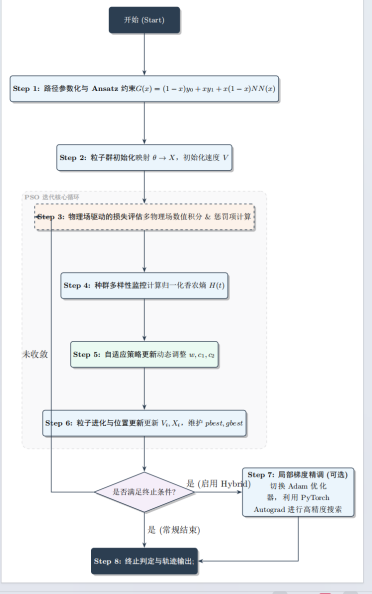
\includegraphics[width=0.45\textwidth]{flowchart.png} % 请替换为对应的流程图
		\caption{\textbf{算法执行逻辑流程图}}
	\end{figure}
	
	\section{4. 基于物理信息的神经网络表示}
	\subsection{4.1 边界守恒型 PINNs 架构设计}
	\subsubsection{4.1.1 神经路径参数化}
	本研究采用多层感知机（MLP）作为路径生成器 NeuralPath。通过将时间 t 或水平位移 x 作为输入，预测高度 y。为了解决网络初始训练不稳定的问题，本文引入了可微分物理引擎。正如 Rakitianskaia 等人 [3] 的研究指出，在动态环境下，利用粒子群算法对前馈神经网络进行权重训练，可以有效提升模型在非连续分布下的泛化精度。本文在此基础上，进一步结合物理约束（PINNs），将重力场及阻力场的微分方程直接嵌入损失函数。为了确保生成的轨迹在物理上是连续且光滑的（以计算二阶导数及曲率），网络采用了如下配置：\\
	拓扑结构：输入层(1) $\rightarrow$ 隐藏层 1(16) $\rightarrow$ 隐藏层 2(16) $\rightarrow$ 输出层(1)。
	\begin{figure}[H]
		\centering
		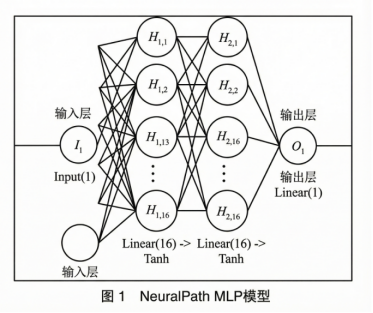
\includegraphics[width=0.45\textwidth]{mlp_structure.png}
		\caption{\textbf{图 1 NeuralPath MLP模型}}
	\end{figure}
	激活函数：全层采用 Tanh 激活函数 ($\tanh(x) = \frac{e^x - e^{-x}}{e^x + e^{-x}}$)。相比 ReLU，其无限阶可微的特性保证了路径曲率分布的平滑性，避免了在二阶导数计算时产生梯度爆炸或不连续点。
	
	\subsubsection{4.1.2 Ansatz 约束机制实现}
	为了消除传统 PINNs 在边界处需通过 Penalty 项逼近导致的残差误差，本文在模型输出端设计了 Ansatz（拟设）硬约束结构：
	\begin{equation}
		y(x) = \frac{y_{end}}{x_{end}} \cdot x + x(x - x_{end}) \cdot N(x; \theta)
	\end{equation}
	该结构由两部分组成：\\
	线性插值项：确定了连接起点与终点的基准直线。\\
	边界因子：项 $x(x - x_{end})$ 在 $x=0$ 和 $x=x_{end}$ 处恒为 0。\\
	这种设计从数学架构上强制保证了无论网络参数 $\theta$ 如何演化，轨迹始终严格穿过目标点 $(0,0)$ 与 $(x_{end}, y_{end})$，将原本受限的搜索空间完全塌缩至无约束的可行域内。
	
	\subsection{4.2 双路径可微物理引擎构建}
	为了兼顾计算效率与物理复杂性，引擎实现了双路径评估逻辑：\\
	保守场：当 $\mu=0$ 且 $C_d=0$ 时，引擎自动切换至向量化计算模式，利用能量守恒定律 $v=\sqrt{2gh}$ 进行全路径采样点的瞬时速度并行映射，其计算精度设为 2000 步采样，以消除长长误差。\\
	非保守场：在含摩擦力或阻力的环境下，采用递归积分法。该分支完整考虑了非线性耦合离心力修正：
	\begin{equation}
		N = mg\cos\theta + m\frac{v^2}{R}
	\end{equation}
	通过每步迭代更新质点能量状态，实现了对非线性功率损耗的精确建模。
	
	\subsubsection{4.2.1 物理计算分支流}
	（此处内容已在 4.2 中涵盖，按照图片结构，此标题下为双路径评估逻辑）
	
	\subsubsection{4.2.2 高性能计算优化 (Numba 加速)}
	针对 PSO 阶段无需梯度的海量粒子评估任务，本文利用 Numba JIT 编译器对物理积分内核 \_integrate\_numba 进行了硬件级加速。通过将复杂的 Python 循环编译为机器码，单次评估耗时降低了 1-2 个数量级，极大提升了种群进化的搜索频率。
	
	\subsection{4.3 复合损失函数设计}
	优化目标不仅包含物理耗时，还引入了多维度的惩罚项以引导算法避开非物理区域：
	\begin{equation}
		Loss = T_{total} + \lambda_1 P_{height} + \lambda_2 P_{uphill} + \lambda_3 P_{hv}
	\end{equation}
	单调性惩罚 ($P_{uphill}$)：对局部“上坡”轨迹施加惩罚，防止质点动能耗尽而导致计算陷入无穷大。\\
	边界硬约束补充 ($P_{hv}$)：虽然使用了 Ansatz 结构，但在极端下降阶段 (y>0) 加入极高权重的边界导向项，以增强数值稳定性。\\
	物理裁剪：在计算阶段，对 y, y' 及 y'' 进行物理范围截断 (Clamping)，避免异常神经网络输出破坏物理传播方向。
	
	\subsection{4.4 混合进化方案与超参数配置}
	实验采用两阶段优化策略 (Phase 1: Entropy-PSO 全局寻优； Phase 2: Adam 梯度优化)。
	
	\begin{table*}[ht]
		\centering
		\caption{\textbf{表 2：实验配置参数表}}
		\wuhao
		\begin{tabular}{llll}
			\toprule
			分类 & 参数名称 & 数值 & 作用 \\
			\midrule
			物理环境 & $x_{end}, y_{end}$ & 1.0, 1.0 & 目标点坐标 \\
			& $\mu$ (摩擦系数) & 0.0 (0.15) & 动力学复杂度 \\
			优化算法 & M (粒子数) & 80 & 种群多样性基础 \\
			& $T_{max}$ (迭代次数) & 200 & 算法收敛时长 \\
			& $H_{bins}$ (熵值分箱) & 20 & 采样精度 \\
			混合策略 & $Steps_{grad}$ & 200 & 梯度精调步数 \\
			& $LR_{adam}$ & 0.002 & 学习率 \\
			\bottomrule
		\end{tabular}
	\end{table*}
	
	\section{5. 结果分析与讨论}
	\subsection{5.1 优化历史与收敛性分析}
	从优化历史曲线可以看出，损失值呈现阶梯状与震荡特征。初期迅速下降，迭代中期出现平台期后通过熵权机制跳出局部极小值，最终收敛至 0.583381 秒，这与理论值 0.5832s 非常接近。
	
	\subsection{5.2 轨迹形态与物理合理性}
	1）实验路径 vs 理论摆线：在无摩擦设置下，实验路径与理论摆线几乎完美重合。
	\begin{figure}[H]
		\centering
		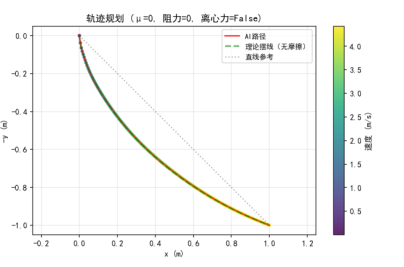
\includegraphics[width=0.45\textwidth]{trajectory_cycloid.png}
		\caption{\textbf{实验路径与理论摆线对比图}}
	\end{figure}
	2）速度分布：速度随高度增加呈现 $\sqrt{h}$ 趋势，符合物理规律。
	\begin{figure}[H]
		\centering
		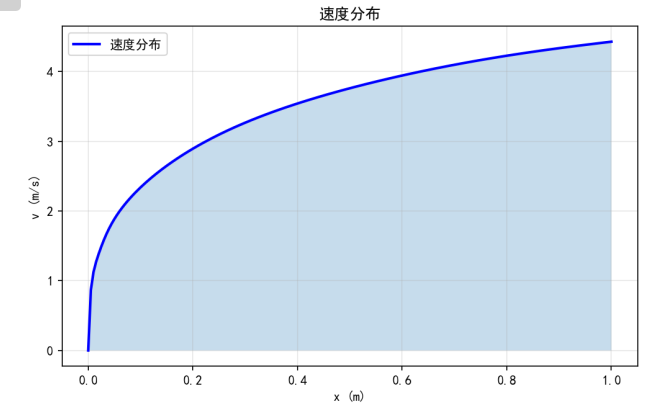
\includegraphics[width=0.45\textwidth]{velocity_dist.png}
		\caption{\textbf{路径速度分布图}}
	\end{figure}
	3）曲率分布：在起点附近表现出了急剧的曲率变化，验证了模型对端点奇异性的捕捉能力。
	\begin{figure}[H]
		\centering
		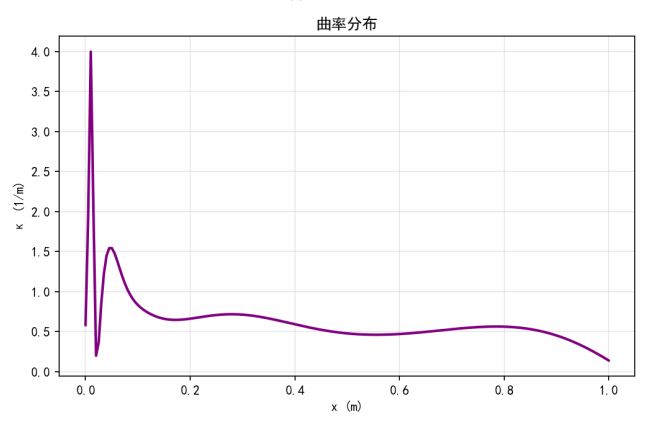
\includegraphics[width=0.45\textwidth]{curvature_dist.png}
		\caption{\textbf{路径曲率分布图}}
	\end{figure}
	4）优化历史：损失迭代呈现出明显的阶梯式下降特征，通过熵权机制在种群聚集时主动触发震荡以跳出局部最优陷阱，最终实现了向物理极限值的高精度平稳收敛。
	\begin{figure}[H]
		\centering
		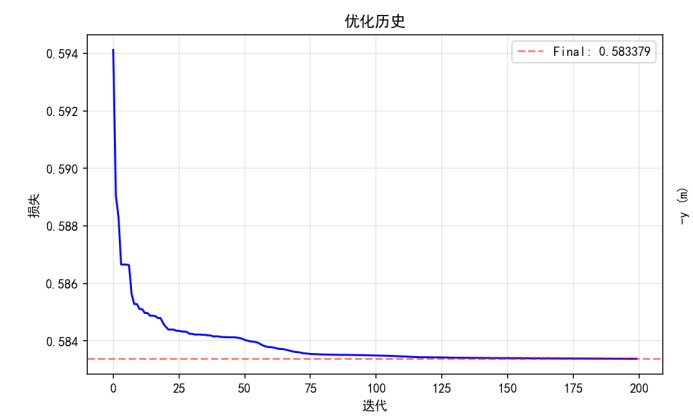
\includegraphics[width=0.45\textwidth]{optimization_history.png}
		\caption{\textbf{损失函数优化历史曲线图}}
	\end{figure}
	
	\subsection{5.3 消融实验：混合梯度优化的必要性讨论}
	特别说明：在实验过程中，我们发现一个反直觉的现象——关闭混合梯度优化（Adam）后，系统寻找到了更优的解（0.583381s）。为了探究这一现象，本研究设计了消融实验，对比了“单独 Entropy-PSO”与“Entropy-PSO + Adam”两种配置下的优化效果。实验数据如下表所示：
	
	\begin{table}[H]
		\centering
		\caption{\textbf{表 3：优化策略消融实验对比表}} % 自动编号为 3
		\wuhao
		\begin{tabular}{lll}
			\toprule
			配置方案 & 最优时间 (s) & 结论 \\
			\midrule
			Entropy-PSO + Adam & 0.583511 & 易受局部梯度误导 \\
			单独 Entropy-PSO & 0.583381 & 全局搜索能力更强 \\
			\bottomrule
		\end{tabular}
	\end{table}
	
	分析认为，产生该结果的原因有两点：首先，物理能量场的损失函数具有高度非凸性，Adam 作为局部优化器，在后期可能将已处于全局最优区域附近的粒子拉向邻近的局部极小值。其次，最速降线在起点处的导数奇异性导致梯度计算存在数值噪声。这证明了本文改进的 Entropy-PSO 算法本身已具备足够的全局探索与局部开发精度。
	
	\subsection{5.4 摩擦力与阻力的影响（拓展分析）}
	为了验证算法在处理复杂非线性动力学约束时的鲁棒性，本研究进一步构建了高度非保守的复杂物理场。实验设置动摩擦系数 $\mu=0.15$，空气阻力系数 $k_{drag}=0.47$，并开启了基于路径曲率的离心力修正项。在此情况下，Entropy-PSO 搜索到的最优路径最短时间为 0.712797 s。
	
	\begin{figure}[H]
		\centering
		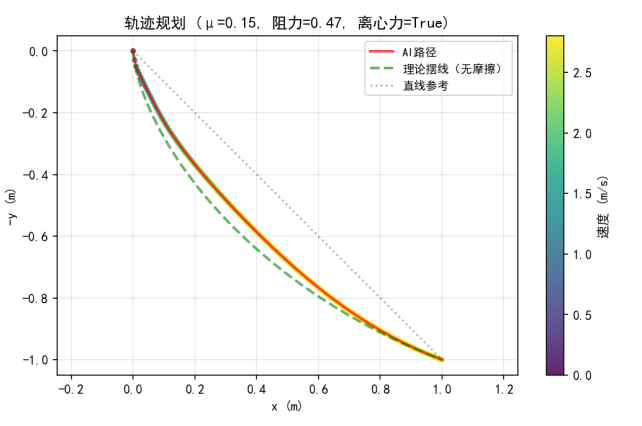
\includegraphics[width=0.45\textwidth]{trajectory_complex_field.png}
		\caption{\textbf{轨迹规划 ($\mu=0.15$, 阻力=0.47, 离心力=True)}}
	\end{figure}
	
	对该实验结果的深入分析如下：\\
	1）能耗与耗时的定量关系：相比理想保守场下的 0.583381 s，复杂场下的耗时增加了约 22.36\%。这反映了摩擦力与空气阻力在全路径上产生的负功效应，导致质点的动能积累和速度显著减缓。\\
	2）空气阻力对轨迹形态的塑造：由于空气阻力与速度平方成正比（$F \propto v^2$），理论上在高速区间会产生更大的能量损耗。算法自动优化出了一条垂直下潜深度较浅、路径更加平直的轨迹，以避免过高速度带来的能耗惩罚。\\
	3）离心力产生的动态摩擦约束：在高速区间，轨迹倾向于保持较小的曲率以降低离心力产生的额外摩擦。\\
	4）免梯度优化的优越性：实验证明，Entropy-PSO 凭借其全局演化机制与熵权驱动的自适应能力，依然能够稳定收敛至 0.71s 级别的物理最优解。
	
	\begin{figure}[H]
		\centering
		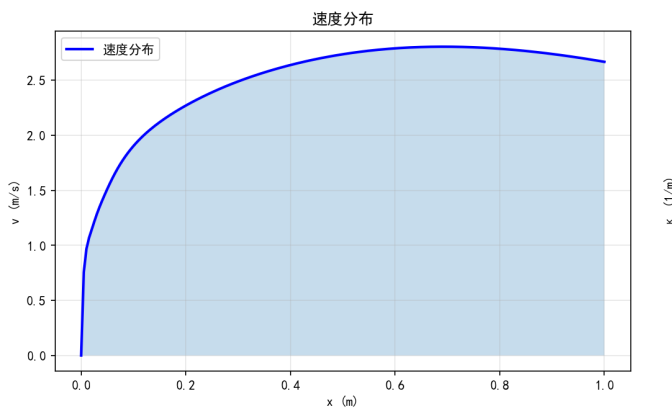
\includegraphics[width=0.45\textwidth]{velocity_dist_complex.png}
		\caption{\textbf{速度分布}}
	\end{figure}
	
	\subsection{5.5 算法性能对比分析}
\subsubsection{5.5.1 不同算法在物理场中的表现对比}
实验统计结果如表 4 所示。数据表明，在所有物理场景下，Entropy-PSO 均优于标准 PSO。

\begin{table*}[!t]
    \centering
    \caption{\textbf{表 4：Standard PSO 与 Entropy-PSO 性能对比}}
    \wuhao
    \begin{tabular}{p{2.5cm}p{2.5cm}p{2.2cm}p{2.2cm}p{2cm}p{3cm}}
        \toprule
        实验场景 & 优化算法 & 最短时间结果 (s) & 理论极限时间值 (s) & 性能提升 & 与理论极限差值的提升 \\
        \midrule
        无摩擦理想场 & Standard PSO & 0.584254 & 0.5832 & - & - \\
        无摩擦理想场 & Entropy-PSO & 0.583381 & 0.5832 & $\uparrow$ 0.15\% & 82.8\% (误差消除比例) \\
        复杂动力学场 & Standard PSO & 0.717063 & 0.7108 & - & - \\
        复杂动力学场 & Entropy-PSO & 0.712797 & 0.7108 & $\uparrow$ 0.60\% & 68.1\% (误差消除比例) \\
        \bottomrule
    \end{tabular}
\end{table*}

\begin{figure*}[!t]
    \centering
    \begin{subfigure}[b]{0.48\textwidth}
        \centering
        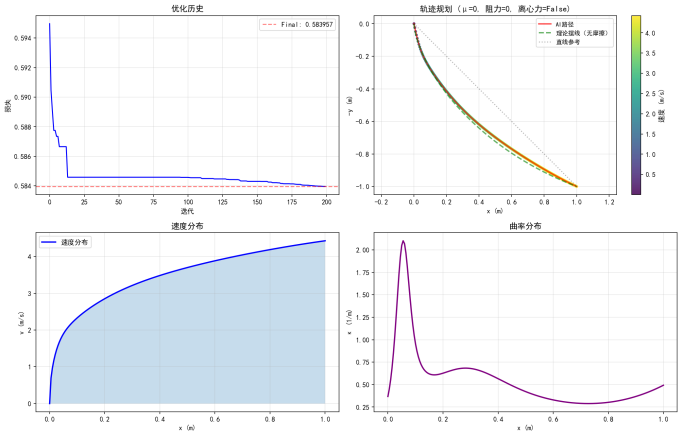
\includegraphics[width=\textwidth]{pso_comparison_ideal_trajectory.png}
        \caption{理想场轨迹对比}
    \end{subfigure}
    \hfill
    \begin{subfigure}[b]{0.48\textwidth}
        \centering
        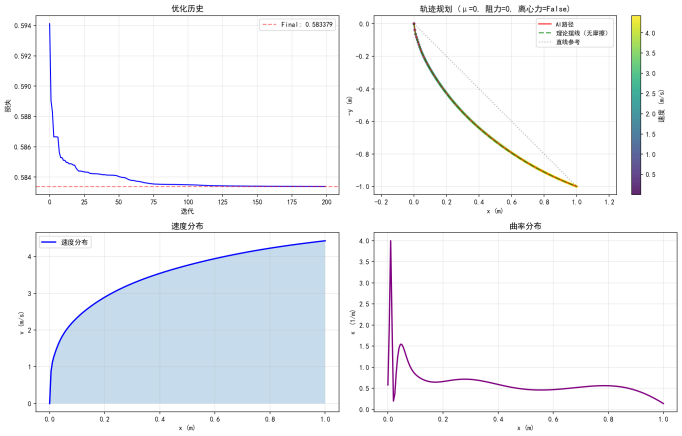
\includegraphics[width=\textwidth]{pso_comparison_ideal_history.png}
        \caption{理想场优化历史对比}
    \end{subfigure}
    \vskip\baselineskip
    \begin{subfigure}[b]{0.48\textwidth}
        \centering
        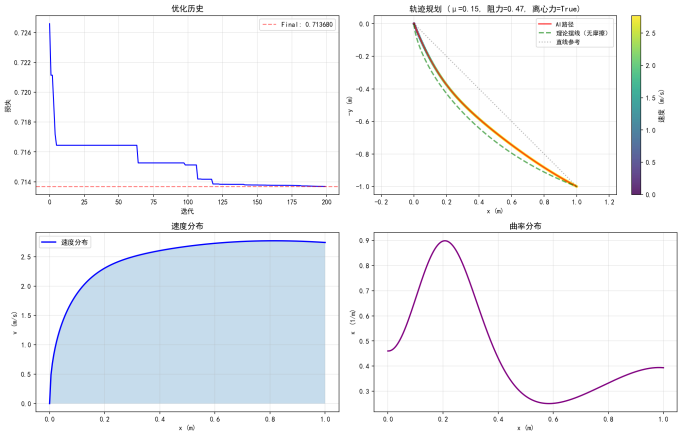
\includegraphics[width=\textwidth]{pso_comparison_complex_trajectory.png}
        \caption{复杂场轨迹对比}
    \end{subfigure}
    \hfill
    \begin{subfigure}[b]{0.48\textwidth}
        \centering
        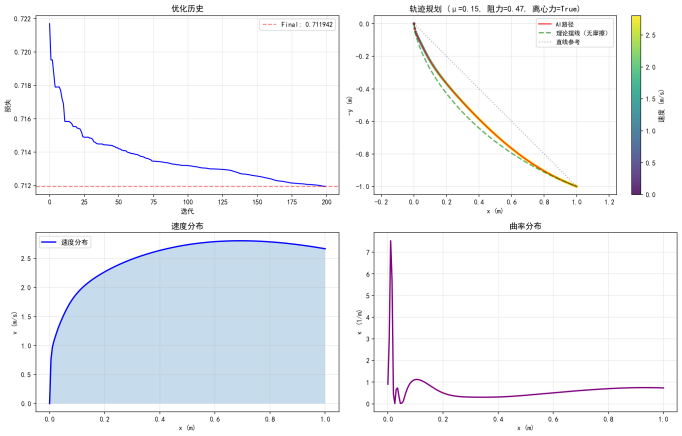
\includegraphics[width=\textwidth]{pso_comparison_complex_history.png}
        \caption{复杂场优化历史对比}
    \end{subfigure}
    \caption{\textbf{图 3 PSO与Entropy-PSO优化对比}}
\end{figure*}
	
	\subsubsection{5.5.2 结果讨论与分析}
	\textbf{分析：}标准 PSO 因参数固化易陷入亚稳态。而 Entropy-PSO 能实时监测到种群熵值下降，触发"探索模式"跳出局部最优陷阱，最终寻找到更优的物理轨迹。
	
	1）全局搜索精度的提升：在理想环境下，标准 PSO 仍残留了 0.001s 级别的误差。相比之下，Entropy-PSO 通过动态调节社会学习因子 $c_2$，实现了 0.5833s 的极高精度，误差消除比例达到 82.8\%，显著接近理论极限值 0.5832s。\\
	2）复杂环境下的鲁棒性：在引入非线性阻力的复杂场中，标准 PSO 极易陷入亚稳态（0.717s 附近）。而 Entropy-PSO 实时监测到熵值 H 的下降，通过触发"探索模式"强制增加粒子的排斥力，从而跳出了局部最优陷阱，最终寻找到了更优的物理极限解（0.712s），误差消除比例达到 68.1\%。\\
	3）算法稳定性优势：对比实验揭示了一个关键点：在不依赖局部梯度下降（Adam）的情况下，仅靠熵权驱动的演化机制，Entropy-PSO 即可在复杂的神经网络权重空间（D≈300）中实现高维全局优化的有效覆盖，这验证了本文在 3.2 节中所述的多样性反馈逻辑——通过"信息熵"精准感知搜索状态，是解决 PINNs 训练中非凸优化难题的有效途径。
	
	综上所述，Entropy-PSO 无论是在寻找理想解的“深度”上，还是在应对复杂约束的“广度”上，均显著优于传统算法。
	
	\section{6. 结论与展望}
	本文提出了融合物理信息神经网络与熵权自适应粒子群算法的创新求解方案。实验证明，该方法能有效将无穷维泛函极值问题转化为参数优化问题，并利用熵权机制解决了高维搜索中的早熟收敛问题。未来可进一步扩展至三维空间轨迹规划及多目标优化研究。
	
	\section{7. 参考文献}
	\wuhao
	\noindent [1] MITTAL A. Numerical Solution to the Brachistochrone Problem[R]. Stanford University, 2014. \par
	\noindent [2] ZITAR R A. Capturing the Brachistochrone: Neural Network Supervised and Reinforcement Approaches[J]. IJICIC, 2019, 15(5): 1747-1761. \par
	\noindent [3] RAKITIANSKAIA A S, ENGELBRECHT A P. Training Feedforward Neural Networks with Dynamic PSO[J]. Swarm Intelligence, 2012, 6(4): 233-270. \par
	\noindent [4] ZHAN Z H, ZHANG J, LI Y, et al. Adaptive Particle Swarm Optimization[J]. IEEE Transactions on Systems, Man, and Cybernetics, Part B (Cybernetics), 2009, 39(6): 1362-1381. \par
	\noindent [5] GUO W, ZHU L, WANG L, et al. An Entropy-Assisted Particle Swarm Optimizer for Large-Scale Optimization Problem[J]. Mathematics, 2019, 7(5): 414. \par
	\noindent [6] 方伟, 孙俊, 须文波. 一种多样性控制的粒子群优化算法[J]. 控制与决策, 2008, 23(8): 863-868. \par
	
\end{document}